% !TEX root = z_output/_GoodwillieTalk.tex
\documentclass{beamer}
\usepackage{etex}
\newcommand{\BEAMERMODE}{}
\usepackage{fullpage}
\usepackage{amsmath,amsthm,amssymb}
\usepackage{mathrsfs,nicefrac}
\usepackage{amssymb}
\usepackage{epsfig}
\usepackage[all]{xy}
\usepackage{sseq}
\usepackage{tocloft}
\usepackage{cancel}
\usepackage[strict]{changepage}
\usepackage{color}
\usepackage{tikz}
\usepackage{extpfeil}
\usepackage{version}
%\usepackage{ifthen}
%Used for disabling hyperref
\ifx\dontloadhyperref\undefined
%\usepackage[pdftex,pdfborder={0 0 0 [1 1]}]{hyperref}
\usepackage[pdftex,pdfborder={0 0 .5 [1 1]}]{hyperref}
\else
\providecommand{\texorpdfstring}[2]{#1}
\fi

%>>>>>>>>>>>>>>>>>>>>>>>>>>>>>>
%<<<       Better ToC       <<<
%>>>>>>>>>>>>>>>>>>>>>>>>>>>>>>
\setlength{\cftbeforesecskip}{0.5ex}

%>>>>>>>>>>>>>>>>>>>>>>>>>>>>>>
%<<<      Hyperref mod      <<<
%>>>>>>>>>>>>>>>>>>>>>>>>>>>>>>

%needs more testing
\newcounter{dummyforrefstepcounter}
\newcommand{\labelRIGHTHERE}[1]
{\refstepcounter{dummyforrefstepcounter}\label{#1}}


%>>>>>>>>>>>>>>>>>>>>>>>>>>>>>>
%<<<  Theorem Environments  <<<
%>>>>>>>>>>>>>>>>>>>>>>>>>>>>>>
\ifx\dontloaddefinitionsoftheoremenvironments\undefined
\theoremstyle{plain}
\newtheorem{thm}{Theorem}[section]
\newtheorem*{thm*}{Theorem}
\newtheorem{lem}[thm]{Lemma}
\newtheorem*{lem*}{Lemma}
\newtheorem{prop}[thm]{Proposition}
\newtheorem*{prop*}{Proposition}
\newtheorem{cor}[thm]{Corollary}
\newtheorem*{cor*}{Corollary}
\newtheorem{defprop}[thm]{Definition-Proposition}
\newtheorem*{punchline}{Punchline}

\theoremstyle{definition}
\newtheorem{defn}{Definition}[section]
\newtheorem*{defn*}{Definition}
\newtheorem{exmp}{Example}[section]
\newtheorem*{exmp*}{Example}
\newtheorem{asspt}{Assumption}[section]
\newtheorem{notation}{Notation}[section]
\newtheorem{exercise}{Exercise}[section]
\newtheorem*{fact*}{Fact}
\newtheorem*{rmk*}{Remark}
\newtheorem{fact}{Fact}
\newtheorem*{aside}{Aside}
\newtheorem*{question}{Question}
\newtheorem*{answer}{Answer}

\else\relax\fi

%>>>>>>>>>>>>>>>>>>>>>>>>>>>>>>
%<<<      Fields, etc.      <<<
%>>>>>>>>>>>>>>>>>>>>>>>>>>>>>>
\DeclareSymbolFont{AMSb}{U}{msb}{m}{n}
\DeclareMathSymbol{\N}{\mathbin}{AMSb}{"4E}
\DeclareMathSymbol{\Octonions}{\mathbin}{AMSb}{"4F}
\DeclareMathSymbol{\Z}{\mathbin}{AMSb}{"5A}
\DeclareMathSymbol{\R}{\mathbin}{AMSb}{"52}
\DeclareMathSymbol{\Q}{\mathbin}{AMSb}{"51}
\DeclareMathSymbol{\PP}{\mathbin}{AMSb}{"50}
\DeclareMathSymbol{\I}{\mathbin}{AMSb}{"49}
\DeclareMathSymbol{\C}{\mathbin}{AMSb}{"43}
\DeclareMathSymbol{\A}{\mathbin}{AMSb}{"41}
\DeclareMathSymbol{\F}{\mathbin}{AMSb}{"46}
\DeclareMathSymbol{\Quaternions}{\mathbin}{AMSb}{"48}


%>>>>>>>>>>>>>>>>>>>>>>>>>>>>>>
%<<<       Operators        <<<
%>>>>>>>>>>>>>>>>>>>>>>>>>>>>>>
\DeclareMathOperator{\ad}{\textbf{ad}}
\DeclareMathOperator{\coker}{coker}
\renewcommand{\ker}{\textup{ker}\,}
\DeclareMathOperator{\End}{End}
\DeclareMathOperator{\Aut}{Aut}
\DeclareMathOperator{\Hom}{Hom}
\DeclareMathOperator{\Maps}{Maps}
\DeclareMathOperator{\Mor}{Mor}
\DeclareMathOperator{\Gal}{Gal}
\DeclareMathOperator{\Ext}{Ext}
\DeclareMathOperator{\Tor}{Tor}
\DeclareMathOperator{\Map}{Map}
\DeclareMathOperator{\Der}{Der}
\DeclareMathOperator{\Rad}{Rad}
\DeclareMathOperator{\rank}{rank}
\DeclareMathOperator{\ArfInvariant}{Arf}
\DeclareMathOperator{\KervaireInvariant}{Ker}
\DeclareMathOperator{\im}{im}
\DeclareMathOperator{\coim}{coim}
\DeclareMathOperator{\trace}{tr}
\DeclareMathOperator{\supp}{supp}
\DeclareMathOperator{\ann}{ann}
\DeclareMathOperator{\spec}{Spec}
\DeclareMathOperator{\proj}{Proj}
\DeclareMathOperator{\fiber}{F}
\DeclareMathOperator{\cofiber}{C}
\DeclareMathOperator{\cone}{cone}
\DeclareMathOperator{\Skel}{Sk}
\DeclareMathOperator{\conn}{conn}
\DeclareMathOperator{\colim}{colim}
\DeclareMathOperator{\limit}{lim}

%>>>>>>>>>>>>>>>>>>>>>>>>>>>>>>
%<<<   Cohomology Theories  <<<
%>>>>>>>>>>>>>>>>>>>>>>>>>>>>>>
\DeclareMathOperator{\KR}{{K\R}}
\DeclareMathOperator{\KO}{{KO}}
\DeclareMathOperator{\K}{{K}}
\DeclareMathOperator{\OmegaO}{{\Omega_{\Octonions}}}

%>>>>>>>>>>>>>>>>>>>>>>>>>>>>>>
%<<<   Algebraic Geometry   <<<
%>>>>>>>>>>>>>>>>>>>>>>>>>>>>>>
\DeclareMathOperator{\Spec}{Spec}
\DeclareMathOperator{\Proj}{Proj}
\DeclareMathOperator{\Sing}{Sing}
\DeclareMathOperator{\shfHom}{\mathscr{H}\textit{\!\!om}}
\newcommand{\WeilDivisors}{\textup{Div}}
\newcommand{\CartierDivisors}{\textup{CaDiv}}
\newcommand{\PrincipalWeilDivisors}{\textup{PrDiv}}
\newcommand{\LocallyPrincipalWeilDivisors}{\textup{LPDiv}}
\newcommand{\PrincipalCartierDivisors}{\textup{PrCaDiv}}
\newcommand{\DivisorClass}{\textup{Cl}}
\newcommand{\CartierClass}{\textup{CaCl}}
\newcommand{\Picard}{\textup{Pic}}
\DeclareMathOperator{\Frob}{Frob}


%>>>>>>>>>>>>>>>>>>>>>>>>>>>>>>
%<<<  Mathematical Objects  <<<
%>>>>>>>>>>>>>>>>>>>>>>>>>>>>>>
\newcommand{\sll}{\mathfrak{sl}}
\newcommand{\gl}{\mathfrak{gl}}
\newcommand{\GL}{\mbox{GL}}
\newcommand{\PGL}{\mbox{PGL}}
\newcommand{\SL}{\mbox{SL}}
\newcommand{\Mat}{\mbox{Mat}}
\newcommand{\Gr}{\textup{Gr}}
\newcommand{\Squ}{\textup{Sq}}
\newcommand{\catSet}{\textit{Sets}}
\newcommand{\RP}{{\R\PP}}
\newcommand{\CP}{{\C\PP}}
\newcommand{\Steen}{\mathscr{A}}
\newcommand{\Orth}{\textup{\textbf{O}}}

%>>>>>>>>>>>>>>>>>>>>>>>>>>>>>>
%<<<  Mathematical Symbols  <<<
%>>>>>>>>>>>>>>>>>>>>>>>>>>>>>>
\newcommand{\DASH}{\textup{---}}
\newcommand{\op}{\textup{op}}
\newcommand{\ob}{\textup{ob}\,}
\newcommand{\ho}{\textup{ho}}
\newcommand{\st}{\textup{st}}
\newcommand{\id}{\textup{id}}
\newcommand{\Bullet}{\ensuremath{\bullet} }

%>>>>>>>>>>>>>>>>>>>>>>>>>>>>>>
%<<<      Some Arrows       <<<
%>>>>>>>>>>>>>>>>>>>>>>>>>>>>>>
\let\shortmapsto\mapsto
\let\mapsto\longmapsto
\newcommand{\mapsfrom}{\,\reflectbox{$\mapsto$}\ }
\newcommand{\bigrightsquig}{\scalebox{2}{\ensuremath{\rightsquigarrow}}}
\newcommand{\bigleftsquig}{\reflectbox{\scalebox{2}{\ensuremath{\rightsquigarrow}}}}

%\newcommand{\cofibration}{\xhookrightarrow{\phantom{\ \,{\sim\!}\ \ }}}
%\newcommand{\fibration}{\xtwoheadrightarrow{\phantom{\sim\!}}}
%\newcommand{\acycliccofibration}{\xhookrightarrow{\ \,{\sim\!}\ \ }}
%\newcommand{\acyclicfibration}{\xtwoheadrightarrow{\sim\!}}
%\newcommand{\leftcofibration}{\xhookleftarrow{\phantom{\ \,{\sim\!}\ \ }}}
%\newcommand{\leftfibration}{\xtwoheadleftarrow{\phantom{\sim\!}}}
%\newcommand{\leftacycliccofibration}{\xhookleftarrow{\ \ {\sim\!}\,\ }}
%\newcommand{\leftacyclicfibration}{\xtwoheadleftarrow{\sim\!}}
%\newcommand{\weakequiv}{\xrightarrow{\ \,\sim\,\ }}
%\newcommand{\leftweakequiv}{\xleftarrow{\ \,\sim\,\ }}

\newcommand{\cofibration}
{\xhookrightarrow{\phantom{\ \,{\raisebox{-.3ex}[0ex][0ex]{\scriptsize$\sim$}\!}\ \ }}}
\newcommand{\fibration}
{\xtwoheadrightarrow{\phantom{\raisebox{-.3ex}[0ex][0ex]{\scriptsize$\sim$}\!}}}
\newcommand{\acycliccofibration}
{\xhookrightarrow{\ \,{\raisebox{-.55ex}[0ex][0ex]{\scriptsize$\sim$}\!}\ \ }}
\newcommand{\acyclicfibration}
{\xtwoheadrightarrow{\raisebox{-.6ex}[0ex][0ex]{\scriptsize$\sim$}\!}}
\newcommand{\leftcofibration}
{\xhookleftarrow{\phantom{\ \,{\raisebox{-.3ex}[0ex][0ex]{\scriptsize$\sim$}\!}\ \ }}}
\newcommand{\leftfibration}
{\xtwoheadleftarrow{\phantom{\raisebox{-.3ex}[0ex][0ex]{\scriptsize$\sim$}\!}}}
\newcommand{\leftacycliccofibration}
{\xhookleftarrow{\ \ {\raisebox{-.55ex}[0ex][0ex]{\scriptsize$\sim$}\!}\,\ }}
\newcommand{\leftacyclicfibration}
{\xtwoheadleftarrow{\raisebox{-.6ex}[0ex][0ex]{\scriptsize$\sim$}\!}}
\newcommand{\weakequiv}
{\xrightarrow{\ \,\raisebox{-.3ex}[0ex][0ex]{\scriptsize$\sim$}\,\ }}
\newcommand{\leftweakequiv}
{\xleftarrow{\ \,\raisebox{-.3ex}[0ex][0ex]{\scriptsize$\sim$}\,\ }}


%>>>>>>>>>>>>>>>>>>>>>>>>>>>>>>
%<<<     Greek Letters      <<<
%>>>>>>>>>>>>>>>>>>>>>>>>>>>>>>
%\newcommand{\oldphi}{\phi}
%\renewcommand{\phi}{\varphi}
\let\oldphi\phi
\let\phi\varphi
\renewcommand{\to}{\longrightarrow}
\newcommand{\eps}{\varepsilon}

%>>>>>>>>>>>>>>>>>>>>>>>>>>>>>>
%<<<  1st-4th & parentheses <<<
%>>>>>>>>>>>>>>>>>>>>>>>>>>>>>>
\newcommand{\first}{^\text{st}}
\newcommand{\second}{^\text{nd}}
\newcommand{\third}{^\text{rd}}
\newcommand{\fourth}{^\text{th}}
\newcommand{\ZEROTH}{$0^\text{th}$ }
\newcommand{\FIRST}{$1^\text{st}$ }
\newcommand{\SECOND}{$2^\text{nd}$ }
\newcommand{\THIRD}{$3^\text{rd}$ }
\newcommand{\FOURTH}{$4^\text{th}$ }
\newcommand{\iTH}{$i^\text{th}$ }
\newcommand{\jTH}{$j^\text{th}$ }
\newcommand{\nTH}{$n^\text{th}$ }

%>>>>>>>>>>>>>>>>>>>>>>>>>>>>>>
%<<<    upright commands    <<<
%>>>>>>>>>>>>>>>>>>>>>>>>>>>>>>
\newcommand{\upcol}{\textup{:}}
\newcommand{\upsemi}{\textup{;}}
\providecommand{\lparen}{\textup{(}}
\providecommand{\rparen}{\textup{)}}
\renewcommand{\lparen}{\textup{(}}
\renewcommand{\rparen}{\textup{)}}
\newcommand{\Iff}{\emph{iff} }

%>>>>>>>>>>>>>>>>>>>>>>>>>>>>>>
%<<<     Environments       <<<
%>>>>>>>>>>>>>>>>>>>>>>>>>>>>>>
\newcommand{\squishlist}
{ %\setlength{\topsep}{100pt} doesn't seem to do anything.
  \setlength{\itemsep}{.5pt}
  \setlength{\parskip}{0pt}
  \setlength{\parsep}{0pt}}
\newenvironment{itemise}{
\begin{list}{\textup{$\rightsquigarrow$}}
   {  \setlength{\topsep}{1mm}
      \setlength{\itemsep}{1pt}
      \setlength{\parskip}{0pt}
      \setlength{\parsep}{0pt}
   }
}{\end{list}\vspace{-.1cm}}
\newcommand{\INDENT}{\textbf{}\phantom{space}}
\renewcommand{\INDENT}{\rule{.7cm}{0cm}}

\newcommand{\itm}[1][$\rightsquigarrow$]{\item[{\makebox[.5cm][c]{\textup{#1}}}]}

\newcommand{\rednote}[1]{{\color{red}#1}\scalebox{.1}{rednote}}
\newcommand{\bluenote}[1]{{\color{blue}#1}\scalebox{.1}{rednote}}
\newcommand{\funcdef}[4]{\begin{align*}
#1&\to #2\\
#3&\mapsto#4
\end{align*}}

%\newcommand{\comment}[1]{}

%>>>>>>>>>>>>>>>>>>>>>>>>>>>>>>
%<<<       Categories       <<<
%>>>>>>>>>>>>>>>>>>>>>>>>>>>>>>
\newcommand{\Ens}{{\mathscr{E}ns}}
\DeclareMathOperator{\Sheaves}{{\mathsf{Shf}}}
\DeclareMathOperator{\Presheaves}{{\mathsf{PreShf}}}
\DeclareMathOperator{\Varieties}{{\mathsf{Var}}}
\DeclareMathOperator{\Schemes}{{\mathsf{Sch}}}
\DeclareMathOperator{\Rings}{{\mathsf{Rings}}}
\DeclareMathOperator{\AbGp}{{\mathsf{AbGp}}}
\DeclareMathOperator{\Modules}{{\mathsf{\!-Mod}}}
\DeclareMathOperator{\QuasiCoherent}{{\mathsf{QCoh}}}
\DeclareMathOperator{\Coherent}{{\mathsf{Coh}}}
\DeclareMathOperator{\GSW}{{\mathcal{SW}^G}}
\DeclareMathOperator{\Burnside}{{\mathsf{Burn}}}
\DeclareMathOperator{\GSet}{{G\mathsf{Set}}}
\DeclareMathOperator{\FinGSet}{{G\mathsf{Set}^\textup{fin}}}
\DeclareMathOperator{\HSet}{{H\mathsf{Set}}}
\DeclareMathOperator{\Cat}{{\mathsf{Cat}}}
\DeclareMathOperator{\Orb}{{\mathsf{Orb}}}
\DeclareMathOperator{\Set}{{\mathsf{Set}}}
\DeclareMathOperator{\sSet}{{\mathsf{sSet}}}
\DeclareMathOperator{\Top}{{\mathsf{Top}}}
\DeclareMathOperator{\GSpectra}{{G-\mathsf{Spectra}}}

%>>>>>>>>>>>>>>>>>>>>>>>>>>>>>>
%<<<     Script Letters     <<<
%>>>>>>>>>>>>>>>>>>>>>>>>>>>>>>
\newcommand{\scrQ}{\mathscr{Q}}
\newcommand{\scrW}{\mathscr{W}}
\newcommand{\scrE}{\mathscr{E}}
\newcommand{\scrR}{\mathscr{R}}
\newcommand{\scrT}{\mathscr{T}}
\newcommand{\scrY}{\mathscr{Y}}
\newcommand{\scrU}{\mathscr{U}}
\newcommand{\scrI}{\mathscr{I}}
\newcommand{\scrO}{\mathscr{O}}
\newcommand{\scrP}{\mathscr{P}}
\newcommand{\scrA}{\mathscr{A}}
\newcommand{\scrS}{\mathscr{S}}
\newcommand{\scrD}{\mathscr{D}}
\newcommand{\scrF}{\mathscr{F}}
\newcommand{\scrG}{\mathscr{G}}
\newcommand{\scrH}{\mathscr{H}}
\newcommand{\scrJ}{\mathscr{J}}
\newcommand{\scrK}{\mathscr{K}}
\newcommand{\scrL}{\mathscr{L}}
\newcommand{\scrZ}{\mathscr{Z}}
\newcommand{\scrX}{\mathscr{X}}
\newcommand{\scrC}{\mathscr{C}}
\newcommand{\scrV}{\mathscr{V}}
\newcommand{\scrB}{\mathscr{B}}
\newcommand{\scrN}{\mathscr{N}}
\newcommand{\scrM}{\mathscr{M}}

%>>>>>>>>>>>>>>>>>>>>>>>>>>>>>>
%<<<     Fractur Letters    <<<
%>>>>>>>>>>>>>>>>>>>>>>>>>>>>>>
\newcommand{\frakQ}{\mathfrak{Q}}
\newcommand{\frakW}{\mathfrak{W}}
\newcommand{\frakE}{\mathfrak{E}}
\newcommand{\frakR}{\mathfrak{R}}
\newcommand{\frakT}{\mathfrak{T}}
\newcommand{\frakY}{\mathfrak{Y}}
\newcommand{\frakU}{\mathfrak{U}}
\newcommand{\frakI}{\mathfrak{I}}
\newcommand{\frakO}{\mathfrak{O}}
\newcommand{\frakP}{\mathfrak{P}}
\newcommand{\frakA}{\mathfrak{A}}
\newcommand{\frakS}{\mathfrak{S}}
\newcommand{\frakD}{\mathfrak{D}}
\newcommand{\frakF}{\mathfrak{F}}
\newcommand{\frakG}{\mathfrak{G}}
\newcommand{\frakH}{\mathfrak{H}}
\newcommand{\frakJ}{\mathfrak{J}}
\newcommand{\frakK}{\mathfrak{K}}
\newcommand{\frakL}{\mathfrak{L}}
\newcommand{\frakZ}{\mathfrak{Z}}
\newcommand{\frakX}{\mathfrak{X}}
\newcommand{\frakC}{\mathfrak{C}}
\newcommand{\frakV}{\mathfrak{V}}
\newcommand{\frakB}{\mathfrak{B}}
\newcommand{\frakN}{\mathfrak{N}}
\newcommand{\frakM}{\mathfrak{M}}

\newcommand{\frakq}{\mathfrak{q}}
\newcommand{\frakw}{\mathfrak{w}}
\newcommand{\frake}{\mathfrak{e}}
\newcommand{\frakr}{\mathfrak{r}}
\newcommand{\frakt}{\mathfrak{t}}
\newcommand{\fraky}{\mathfrak{y}}
\newcommand{\fraku}{\mathfrak{u}}
\newcommand{\fraki}{\mathfrak{i}}
\newcommand{\frako}{\mathfrak{o}}
\newcommand{\frakp}{\mathfrak{p}}
\newcommand{\fraka}{\mathfrak{a}}
\newcommand{\fraks}{\mathfrak{s}}
\newcommand{\frakd}{\mathfrak{d}}
\newcommand{\frakf}{\mathfrak{f}}
\newcommand{\frakg}{\mathfrak{g}}
\newcommand{\frakh}{\mathfrak{h}}
\newcommand{\frakj}{\mathfrak{j}}
\newcommand{\frakk}{\mathfrak{k}}
\newcommand{\frakl}{\mathfrak{l}}
\newcommand{\frakz}{\mathfrak{z}}
\newcommand{\frakx}{\mathfrak{x}}
\newcommand{\frakc}{\mathfrak{c}}
\newcommand{\frakv}{\mathfrak{v}}
\newcommand{\frakb}{\mathfrak{b}}
\newcommand{\frakn}{\mathfrak{n}}
\newcommand{\frakm}{\mathfrak{m}}

%>>>>>>>>>>>>>>>>>>>>>>>>>>>>>>
%<<<  Caligraphic Letters   <<<
%>>>>>>>>>>>>>>>>>>>>>>>>>>>>>>
\newcommand{\calQ}{\mathcal{Q}}
\newcommand{\calW}{\mathcal{W}}
\newcommand{\calE}{\mathcal{E}}
\newcommand{\calR}{\mathcal{R}}
\newcommand{\calT}{\mathcal{T}}
\newcommand{\calY}{\mathcal{Y}}
\newcommand{\calU}{\mathcal{U}}
\newcommand{\calI}{\mathcal{I}}
\newcommand{\calO}{\mathcal{O}}
\newcommand{\calP}{\mathcal{P}}
\newcommand{\calA}{\mathcal{A}}
\newcommand{\calS}{\mathcal{S}}
\newcommand{\calD}{\mathcal{D}}
\newcommand{\calF}{\mathcal{F}}
\newcommand{\calG}{\mathcal{G}}
\newcommand{\calH}{\mathcal{H}}
\newcommand{\calJ}{\mathcal{J}}
\newcommand{\calK}{\mathcal{K}}
\newcommand{\calL}{\mathcal{L}}
\newcommand{\calZ}{\mathcal{Z}}
\newcommand{\calX}{\mathcal{X}}
\newcommand{\calC}{\mathcal{C}}
\newcommand{\calV}{\mathcal{V}}
\newcommand{\calB}{\mathcal{B}}
\newcommand{\calN}{\mathcal{N}}
\newcommand{\calM}{\mathcal{M}}

%>>>>>>>>>>>>>>>>>>>>>>>>>>>>>>
%<<<<<<<<<DEPRECIATED<<<<<<<<<<
%>>>>>>>>>>>>>>>>>>>>>>>>>>>>>>

%%% From Kac's template
% 1-inch margins, from fullpage.sty by H.Partl, Version 2, Dec. 15, 1988.
%\topmargin 0pt
%\advance \topmargin by -\headheight
%\advance \topmargin by -\headsep
%\textheight 9.1in
%\oddsidemargin 0pt
%\evensidemargin \oddsidemargin
%\marginparwidth 0.5in
%\textwidth 6.5in
%
%\parindent 0in
%\parskip 1.5ex
%%\renewcommand{\baselinestretch}{1.25}

%%% From the net
%\newcommand{\pullbackcorner}[1][dr]{\save*!/#1+1.2pc/#1:(1,-1)@^{|-}\restore}
%\newcommand{\pushoutcorner}[1][dr]{\save*!/#1-1.2pc/#1:(-1,1)@^{|-}\restore}









\usetikzlibrary{arrows,positioning}
\usetikzlibrary{decorations.markings}
\usetikzlibrary{calc}
\tikzset{
 >=stealth',
 shorten <=-5pt,
 shorten >=-5pt,
 shape=circle
}

\newcommand{\tallstrut}{\rule[-.5em]{0pt}{1.75em}}
\newcommand{\TF}{\raisebox{.091em}{$\therefore$}\,}
\newcommand\ST{\rule[-.25em]{0pt}{1.25em}}
\newcommand{\dist}{\ell}
\newcommand{\cartesianness}{\textup{cart}}
\excludeversion{push vs pull}

\def\excludeversion#1{\includeversion{#1}}
\excludeversion{partial derivatives}
\excludeversion{Iterated Lipschitz conditions}
\excludeversion{distances in Top}
\includeversion{functors appear}
\excludeversion{Excisivity and Analyticity}
\excludeversion{II.1.6}
\excludeversion{II.1.20}
\excludeversion{II.1.22}
\includeversion{III.1.4}
\excludeversion{III.1.5}
\includeversion{III.1.13}

%
%\setbeamercolor{block title}{bg=light blue,fg=blue}%bg=background, fg= foreground
%\setbeamercolor{block body}{bg=yellow,fg=green}%bg=background, fg= foreground
%
%\setbeamertemplate{blocks}[rounded][shadow=true]
%%\setbeamertemplate{blocks}[horizontal shading][left=white!40!black,right=black]
%%\setbeamertemplate{background canvas}[vertical shading][bottom=white,top=structure.fg!25]
%%\setbeamertemplate{sidebar canvas left}[horizontal shading][left=white!40!black,right=black]
%%\usetheme{Malmoe}

\usecolortheme{orchid}


%
%%http://tex.stackexchange.com/questions/13793/beamer-alt-command-like-visible-instead-of-like-only
%\makeatletter
%% Detect mode. mathpalette is used to detect the used math style
%\newcommand<>\Alt[2]{%
%    \begingroup
%    \ifmmode
%        \expandafter\mathpalette
%        \expandafter\math@Alt
%    \else
%        \expandafter\make@Alt
%    \fi
%    {{#1}{#2}{#3}}%
%    \endgroup
%}
%
%% Un-brace the second argument (required because \mathpalette reads the three arguments as one
%\newcommand\math@Alt[2]{\math@@Alt{#1}#2}
%
%% Set the two arguments in boxes. The math style is given by #1. \m@th sets \mathsurround to 0.
%\newcommand\math@@Alt[3]{%
%    \setbox\z@ \hbox{$\m@th #1{#2}$}%
%    \setbox\@ne\hbox{$\m@th #1{#3}$}%
%    \@Alt
%}
%
%% Un-brace the argument
%\newcommand\make@Alt[1]{\make@@Alt#1}
%
%% Set the two arguments into normal boxes
%\newcommand\make@@Alt[2]{%
%    \sbox\z@ {#1}%
%    \sbox\@ne{#2}%
%    \@Alt
%}
%
%% Place one of the two boxes using \rlap and place a \phantom box with the maximum of the two boxes
%\newcommand\@Alt[1]{%
%    \alt#1%
%        {\rlap{\usebox0}}%
%        {\rlap{\usebox1}}%
%    \setbox\tw@\null
%    \ht\tw@\ifnum\ht\z@>\ht\@ne\ht\z@\else\ht\@ne\fi
%    \dp\tw@\ifnum\dp\z@>\dp\@ne\dp\z@\else\dp\@ne\fi
%    \wd\tw@\ifnum\wd\z@>\wd\@ne\wd\z@\else\wd\@ne\fi
%    \box\tw@
%}
%
%\makeatother
%%http://tex.stackexchange.com/questions/13793/beamer-alt-command-like-visible-instead-of-like-only
%
%\newcommand<>{\AltMpages}[2]{\Alt<#1>{\begin{minipage}{\linewidth}#2\end{minipage}}{\begin{minipage}{\linewidth}#3\end{minipage}}}
%
%\newcommand{\MINI}[1]{\begin{minipage}{\linewidth}#1\end{minipage}}



\begin{document}
\title{Calc 101}   
\author{Michael Donovan} 
\date{\today} 

%\frame{\titlepage} 

%\frame{\frametitle{Table of contents}\tableofcontents} 

\begin{partial derivatives}

\section{Section no.1} 
\frame{\frametitle{Partial derivatives} 
\tallstrut Have: $f:\R^n\to\R^n$. Seek: $\Delta_uf(x_{\emptyset })$\\
\vspace{.5cm}
\begin{tikzpicture}[scale=1.2]

\path (0.3,0) node[name=2] {$\phantom{\bullet} $};
\path (1.5-1.5,1)+(7-1+.7,1.8-.3) node[name=3] {$\phantom{\bullet} $};
\path (1.5-1.5,1)+(7+1.3+.5,-.2) node[name=123] {$\phantom{\bullet} $};
\path (7+1.3+.2+.3-1.5,0-.5) node[name=12] {$\phantom{\bullet} $};

\path (0,1) node[name=0d] {$\bullet $};
\path (1,1) node[name=1] {$\bullet $};
\path (0d) node[shape=rectangle,left] {\makebox[0cm][r]{$x_{\emptyset }$}};
\path (1) node[shape=rectangle,right] {$x_{1}$};

\path[->,very thick,white] (0d) edge node[left,font=\footnotesize]{$\phantom{v}$} (2);

\path[->,very thick] (0d) edge node[below,font=\footnotesize]{$u$} (1);

\draw [ |->,dashed, decoration={markings,mark=at position 1 with {\arrow[scale=1.7]{>}}},
    postaction={decorate},
    shorten >=0.4pt
] (3.25,1) -- (4,1);

\path (7-1-1.5,1.5) node[name=0] {$\bullet $};

\path (7+1.3+.2+.3-1.5,1-.5-.1) node[name=1] {$\bullet $};

\path[->,very thick,densely dotted] (0) edge node[above right] {$a_{(f\scrx)}$} (1);

\path (0) node[shape=rectangle,above] {$f(x_{\emptyset })$};
\path (1) node[shape=rectangle,below] {$f(x_{1})$};
\path (0,2.5) node[shape=rectangle] {\underline{$\scrx$}};
\path (4.5,2.5) node[shape=rectangle] {\underline{$f\scrx$}};
\end{tikzpicture}\\
\tallstrut The dotted vector $a_{{(f\scrx)}}$ %(call me $a_X$, and add $x_1,x_2,x_{12}$)
 approximates $ \partial_uf(x_{\emptyset })$.
}
\frame{\frametitle{Partial derivatives} 
\tallstrut Have: $f:\R^n\to\R^n$. Seek: $\Delta_v\Delta_uf(x_{\emptyset })$\\
\vspace{.5cm}
\begin{tikzpicture}[scale=1.2]

\path (1.5-1.5,1)+(7-1+.7,1.8-.3) node[name=3] {$\phantom{\bullet} $};
\path (1.5-1.5,1)+(7+1.3+.5,-.2) node[name=123] {$\phantom{\bullet} $};
\path (7+1.3+.2+.3-1.5,0-.5) node[name=12] {$\phantom{\bullet} $};

\path (0.3,0) node[name=2] {$\bullet $};
\path (1.3,0) node[name=12] {$\bullet $};
\path (0,1) node[name=0d] {$\bullet $};
\path (1,1) node[name=1] {$\bullet $};
\path (0d) node[shape=rectangle,left] {\makebox[0cm][r]{$x_{\emptyset }$}};
\path (1) node[shape=rectangle,right] {$x_{1}$};
\path (2) node[shape=rectangle,left] {$x_{2}$};
\path (12) node[shape=rectangle,right] {$x_{12}$};

\path[->,very thick] (0d) edge node[below,font=\footnotesize]{$u$} (1);
\path[->,very thick] (0d) edge node[left,font=\footnotesize]{$v$} (2);

\path[->] (1) edge (12);
\path[->] (2) edge (12);

\draw [ |->,dashed, decoration={markings,mark=at position 1 with {\arrow[scale=1.7]{>}}},
    postaction={decorate},
    shorten >=0.4pt
] (3.25,1) -- (4,1);

\path (7-1-1.5,1.5) node[name=0] {$\bullet $};

\path (7+1.3+.2+.3-1.5,1-.5-.1) node[name=1] {$\bullet $};
\path (7+0.3-1.5,-0.42) node[name=2] {$\bullet $};

\path (7+1.3+.2+.3-1.5,0-.5) node[name=12] {$\bullet $};

\path let \p1 = (2), \p2 = (1), \p3=(12) in node[name=pull]  at (\x1+\x2-\x3,\y1+\y2-\y3) {$\circ$};

\path[->] (0) edge (1);
\path[->] (0) edge (2);
\path[->] (1) edge (12);
\path[->] (2) edge (12);
\path[->] (pull) edge (1);
\path[->] (pull) edge (2);
\path[->,very thick,densely dotted] (0) edge (pull);

\path (0,2.5) node[shape=rectangle] {\underline{$\scrx$}};
\path (4.5,2.5) node[shape=rectangle] {\underline{$f\scrx$}};
\end{tikzpicture}\\
\tallstrut The dotted vector $a_{{(f\scrx)}}$ approximates $- \partial_v \partial_uf(x_{\emptyset })$.
}

\frame{\frametitle{Partial derivatives} 
\tallstrut Have: $f:\R^n\to\R^n$. Seek: $\Delta_w\Delta_v\Delta_uf(x_{\emptyset })$\\
\vspace{.5cm}
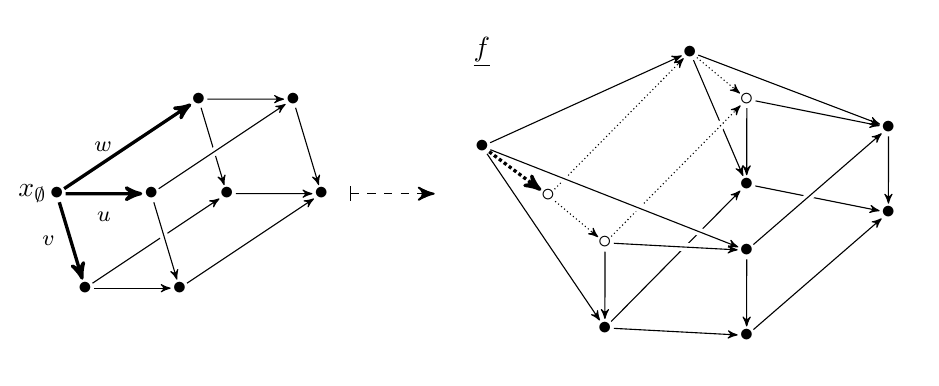
\begin{tikzpicture}[scale=1.2]
\path (0.3,0) node[name=2] {$\bullet $};
\path (1.3,0) node[name=12] {$\bullet $};
\path (0,1) node[name=0d] {$\bullet $};
\path (0d) node[shape=rectangle,left] {\makebox[0cm][r]{$x_{\emptyset }$}};
\path (1,1) node[name=1] {$\bullet $};
\path (1.5,1)+(0.3,0) node[name=23] {$\bullet $};
\path (1.5,1)+(1.3,0) node[name=123] {$\bullet $};
\path (1.5,1)+(0,1) node[name=3] {$\bullet $};
\path (1.5,1)+(1,1) node[name=13] {$\bullet $};

\path[->,very thick] (0d) edge node[below,font=\footnotesize]{$u$} (1);
\path[->,very thick] (0d) edge node[left,font=\footnotesize]{$v$} (2);
\path[->,very thick] (0d) edge node[left,font=\footnotesize]{$w$} (3);

\path[->] (2) edge (12);

\path[->] (3) edge  (23);
\path[->] (3) edge  (13);
\path[->] (13) edge (123);
\path[->] (23) edge (123);


\path[->] (2) edge  (23);
\path[->] (12) edge  (123);

\path[->] (1) edge [-,line width=3pt,draw=white] (12)
			edge (12);
\path[->] (1) edge [-,line width=3pt,draw=white] (13)
			edge (13);

\draw [ |->,dashed, decoration={markings,mark=at position 1 with {\arrow[scale=1.7]{>}}},
    postaction={decorate},
    shorten >=0.4pt
] (3.25,1) -- (4,1);

\path (7-1-1.5,1.5) node[name=0] {$\bullet $};

\path (7+1.3+.2+.3-1.5,1-.5-.1) node[name=1] {$\bullet $};
\path (7+0.3-1.5,-0.42) node[name=2] {$\bullet $};
\path (1.5-1.5,1)+(7-1+.7,1.8-.3) node[name=3] {$\bullet $};

\path (7+1.3+.2+.3-1.5,0-.5) node[name=12] {$\bullet $};
\path (1.5-1.5,1)+(7+0.3,.1) node[name=23] {$\bullet $};
\path (1.5-1.5,1)+(7+1.3+.5,.7) node[name=13] {$\bullet $};

\path (1.5-1.5,1)+(7+1.3+.5,-.2) node[name=123] {$\bullet $};

\path let \p1 = (2), \p2 = (1), \p3=(12) in node[name=pull]  at (\x1+\x2-\x3,\y1+\y2-\y3) {$\circ$};
\path let \p1 = (23), \p2 = (13), \p3=(123) in node[name=pull3]  at (\x1+\x2-\x3,\y1+\y2-\y3) {$\circ$};
\path let \p1 = (3), \p2 = (pull), \p3=(pull3) in node[name=pullpull]  at (\x1+\x2-\x3,\y1+\y2-\y3) {$\circ$};

\path[->] (0) edge (2);
\path[->] (1) edge (12);
\path[->] (2) edge (12);
\path[->] (pull) edge (2);
\path[->,very thick,densely dotted] (0) edge (pullpull);

\path[->] (3) edge (13);
\path[->] (3) edge (23);
\path[->] (13) edge (123);
\path[->] (23) edge (123);
\path[->] (pull3) edge (13);
\path[->] (pull3) edge (23);
\path[->,densely dotted] (3) edge (pull3);
\path[->,densely dotted] (pullpull) edge (pull);
\path[->,densely dotted] (pullpull) edge (3);

\path[->] (0) edge (3);
\path[->] (2) edge (23);
\path[->] (12) edge (123);

\path[->] (pull) edge [-,line width=3pt,draw=white] (pull3);
\path[->,densely dotted] (pull) edge (pull3);
\path[->] (pull) edge [-,line width=3pt,draw=white] (1) edge (1);

\path[->, shorten >=.25cm, shorten <=.25cm] (0) edge [-,line width=3pt,draw=white] (1);
\path[->] (0) edge (1);
\path[->] (1) edge [-,line width=3pt,draw=white] (13) edge (13);


\path (0,2.5) node[shape=rectangle] {\underline{$\scrx$}};
\path (4.5,2.5) node[shape=rectangle] {\underline{$f\scrx$}};
\end{tikzpicture}\\
\tallstrut The dotted vector $a_{{(f\scrx)}}$ approximates $\partial_w \partial_v \partial_uf(x_{\emptyset })$.
}

\end{partial derivatives}
\begin{Iterated Lipschitz conditions}
\frame{\frametitle{A 3-fold Lipschitz condition}
\tallstrut \uncover<1->{Can demand: $|a_{(f\scrx)}|\leq L\cdot|u|\cdot|v|\cdot|w|$ for all \emph{short} $u,v,w$.}\\ %$\partial_w\partial_v\partial_uf(x_{\emptyset })$\\
\vspace{.5cm}
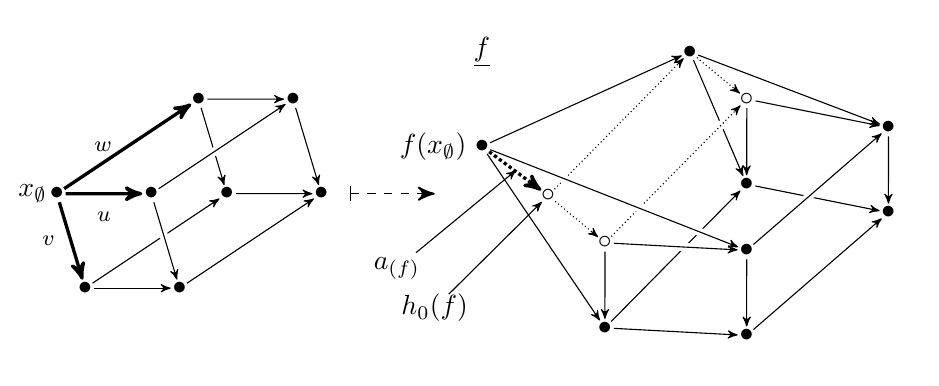
\begin{tikzpicture}[scale=1.2]
\path (0.3,0) node[name=2] {$\bullet $};
\path (1.3,0) node[name=12] {$\bullet $};
\path (0,1) node[name=0d] {$\bullet $};
\path (0d) node[shape=rectangle,left] {\makebox[0cm][r]{$x_{\emptyset }$}};
\path (1,1) node[name=1] {$\bullet $};
\path (1.5,1)+(0.3,0) node[name=23] {$\bullet $};
\path (1.5,1)+(1.3,0) node[name=123] {$\bullet $};
\path (1.5,1)+(0,1) node[name=3] {$\bullet $};
\path (1.5,1)+(1,1) node[name=13] {$\bullet $};

\path[->,very thick] (0d) edge node[below,font=\footnotesize]{$u$} (1);
\path[->,very thick] (0d) edge node[left,font=\footnotesize]{$v$} (2);
\path[->,very thick] (0d) edge node[left,font=\footnotesize]{$w$} (3);

\path[->] (2) edge (12);

\path[->] (3) edge  (23);
\path[->] (3) edge  (13);
\path[->] (13) edge (123);
\path[->] (23) edge (123);


\path[->] (2) edge  (23);
\path[->] (12) edge  (123);

\path[->] (1) edge [-,line width=3pt,draw=white] (12)
			edge (12);
\path[->] (1) edge [-,line width=3pt,draw=white] (13)
			edge (13);

\draw [ |->,dashed, decoration={markings,mark=at position 1 with {\arrow[scale=1.7]{>}}},
    postaction={decorate},
    shorten >=0.4pt
] (3.25,1) -- (4,1);

\path (7-1-1.5,1.5) node[name=0] {$\bullet $};
\path (0) node[left] {$f(x_\emptyset) $};

\path (7+1.3+.2+.3-1.5,1-.5-.1) node[name=1] {$\bullet $};
\path (7+0.3-1.5,-0.42) node[name=2] {$\bullet $};
\path (1.5-1.5,1)+(7-1+.7,1.8-.3) node[name=3] {$\bullet $};

\path (7+1.3+.2+.3-1.5,0-.5) node[name=12] {$\bullet $};
\path (1.5-1.5,1)+(7+0.3,.1) node[name=23] {$\bullet $};
\path (1.5-1.5,1)+(7+1.3+.5,.7) node[name=13] {$\bullet $};

\path (1.5-1.5,1)+(7+1.3+.5,-.2) node[name=123] {$\bullet $};

\path let \p1 = (2), \p2 = (1), \p3=(12) in node[name=pull]  at (\x1+\x2-\x3,\y1+\y2-\y3) {$\circ$};
\path let \p1 = (23), \p2 = (13), \p3=(123) in node[name=pull3]  at (\x1+\x2-\x3,\y1+\y2-\y3) {$\circ$};
\path let \p1 = (3), \p2 = (pull), \p3=(pull3) in node[name=pullpull]  at (\x1+\x2-\x3,\y1+\y2-\y3) {$\circ$};

\path[->] (0) edge (2);
\path[->] (1) edge (12);
\path[->] (2) edge (12);
\path[->] (pull) edge (2);
\path[->,very thick,densely dotted] (0) edge node[name=midedge]{} (pullpull);

\path[->] (3) edge (13);
\path[->] (3) edge (23);
\path[->] (13) edge (123);
\path[->] (23) edge (123);
\path[->] (pull3) edge (13);
\path[->] (pull3) edge (23);
\path[->,densely dotted] (3) edge (pull3);
\path[->,densely dotted] (pullpull) edge (pull);
\path[->,densely dotted] (pullpull) edge (3);

\path[->] (0) edge (3);
\path[->] (2) edge (23);
\path[->] (12) edge (123);

\path[->] (pull) edge [-,line width=3pt,draw=white] (pull3);
\path[->,densely dotted] (pull) edge (pull3);
\path[->] (pull) edge [-,line width=3pt,draw=white] (1) edge (1);

\path[->, shorten >=.25cm, shorten <=.25cm] (0) edge [-,line width=3pt,draw=white] (1);
\path[->] (0) edge (1);
\path[->] (1) edge [-,line width=3pt,draw=white] (13) edge (13);

\path[->] (4,-.21) node[shape=rectangle] {$h_0(f\scrx)$} edge (pullpull);
\path[->, shorten >=-2mm] (3.6,.21) node {$a_{(f\scrx)}$} edge (midedge);
\path (0,2.5) node[shape=rectangle] {\underline{$\scrx$}};
\path (4.5,2.5) node[shape=rectangle] {\underline{$f\scrx$}};
\end{tikzpicture}\\
\tallstrut \uncover<2->{Then $|\partial_w\partial_v\partial_uf|\leq L$ (where it exists) whenever $|u|,|v|,|w|\leq1$.}
%The dotted vector should still approximate $\partial_w \partial_v \partial_uf(x_{\emptyset })$.
}
%
%\frame{\frametitle{Iterated Lipschitz conditions; $E_n(c,\kappa)$}
%$f$ has \underline{$E_n(c,\kappa)$} if ($f$ is $C^\infty$, and)\pause\\
%\begin{center}
%whenever $x_\emptyset ,x_1,\ldots,x_{n+1}\in \R^n$ satisfy $|x_\emptyset -x_i|\leq e^{-\kappa}$,\pause\\
%and $\scrx$ is the cube with $x_\emptyset \rightarrow x_i$ as initial arrows:\pause
%\[|a_{f(\scrx)}|\leq e^c\prod_{i=1}^{n+1}|x_\emptyset -x_i|.\]
%\end{center}\pause
%Then all $(n+1)^\textup{st}$ derivatives are bounded by $e^c$ (where they exist).\pause
%
%\begin{center}{\color{blue}This will define ``stably $n$-excisive functor''!}\end{center}
%}

\frame{\frametitle{Iterated Lipschitz conditions; $E_n(c,\kappa)$}
\begin{block}{Definition}$f$ has \underline{$E_n(c,\kappa)$} if \pause ($f$ is $C^\infty$, and)\pause\\
\begin{center}
whenever $x_\emptyset ,x_1,\ldots,x_{n+1}\in \R^n$ satisfy $|x_\emptyset -x_i|\leq e^{-\kappa}$,\pause\\
and $\scrx$ is the cube with $x_\emptyset \rightarrow x_i$ as initial arrows:\pause
\[|a_{f(\scrx)}|\leq e^c\prod_{i=1}^{n+1}|x_\emptyset -x_i|.\]
\end{center}\end{block}\pause
Then all $(n+1)^\textup{st}$ derivatives are bounded by $e^c$.\pause

\begin{center}{\color{blue}This will define ``stably $n$-excisive functor''!}\end{center}

}

%%% BEGIN: \usebox{\saveboxVUS}
\newsavebox{\saveboxVUS}
\sbox{\saveboxVUS}{
\fbox{\txt{$f$ analytic near $y$}}
}%%% END:  \usebox{\saveboxVUS}
%%% BEGIN: \usebox{\saveboxXLZ}
\newsavebox{\saveboxXLZ}
\sbox{\saveboxXLZ}{
\fbox{\txt{For some $\alpha>0$:\rule[-.5em]{0pt}{.1em}\\$\left|\frac{d^kf}{dx^k}(x)\right|\leq \alpha^{k+1}k!$\\whenever $|x-y|\leq \alpha^{-1}$}}
}%%% END:  \usebox{\saveboxXLZ}
%%% BEGIN: \usebox{\saveboxQWW}
\newsavebox{\saveboxQWW}
\sbox{\saveboxQWW}{
\fbox{\txt{$f$ has $\alpha^{-1}$ as radius\\ of convergence at $y$}}
}%%% END:  \usebox{\saveboxQWW}
%%% BEGIN: \usebox{\saveboxZVB}
\newsavebox{\saveboxZVB}
\sbox{\saveboxZVB}{
\fbox{\txt{For some $q\in\Z$, $\rho\in\Z_{\geq0}$:\rule[-.5em]{0pt}{.1em}\\$f$ has $E_n(n\rho-q,\rho+1)$\\for all $n\geq0$.}}
}%%% END:  \usebox{\saveboxZVB}

\frame{\frametitle{Iterated Lipschitz conditions; $An(\rho)$}
For $f$ a $C^\infty$ function $C\to \R$, where $y\in C\subset \R$:
\[\xymatrix{\uncover<1->{\usebox{\saveboxVUS}}
\only<2->{\ar@{<=>}[rr]}
&&\uncover<2->{\usebox{\saveboxXLZ}}
\only<3->{\ar@{=>}[lld]}
\\
\uncover<3->{\usebox{\saveboxQWW}}&&
\uncover<4->{\usebox{\saveboxZVB}}
\only<4->{\ar@{=>}[u]}%_-{\textup{($\alpha\approx e^{\rho+1}$)}}
\\&\uncover<5->{\makebox[.10cm][c]{{\color{blue}This will define ``$\rho$-analytic functor''!}}}
\only<5->{\ar@(u,l)[ur]}
}\]
}
\end{Iterated Lipschitz conditions}
%<2pc>


\begin{push vs pull}
\frame{%\frametitle{Pushout vs.\ pullback} 
\tallstrut \\%Nice diagram:\\ %$\partial_w\partial_v\partial_uf(x_{\emptyset })$\\
\vspace{.5cm}
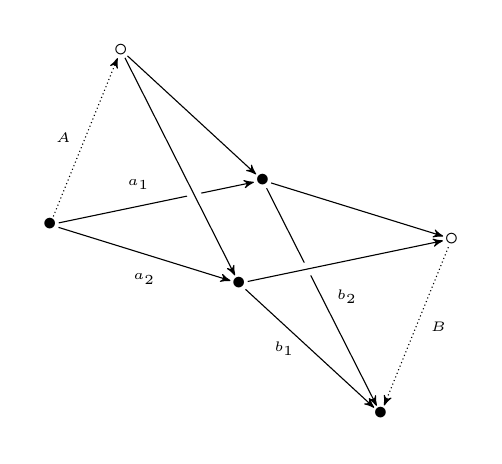
\begin{tikzpicture}[yscale=1.2,xscale=1.5]
%\path (0.3,0) node[name=2] {$\bullet $};
%\path (1.3,0) node[name=12] {$\bullet $};
%\path (0,1) node[name=0d] {$\bullet $};
%\path (0d) node[shape=rectangle,left] {\makebox[0cm][r]{$\scrx_{\emptyset }$}};\pause
%\path (1,1) node[name=1] {$\bullet $};
%\path (1.5,1)+(0.3,0) node[name=23] {$\bullet $};
%\path (1.5,1)+(1.3,0) node[name=123] {$\bullet $};
%\path (1.5,1)+(0,1) node[name=3] {$\bullet $};
%\path (1.5,1)+(1,1) node[name=13] {$\bullet $};
%
%\path[->,very thick] (0d) edge node[below,font=\footnotesize]{$u$} (1);
%\path[->,very thick] (0d) edge node[left,font=\footnotesize]{$v$} (2);
%\path[->,very thick] (0d) edge node[left,font=\footnotesize]{$w$} (3);
%
%\path[->] (2) edge (12);
%
%\path[->] (3) edge  (23);
%\path[->] (3) edge  (13);
%\path[->] (13) edge (123);
%\path[->] (23) edge (123);
%
%
%\path[->] (2) edge  (23);
%\path[->] (12) edge  (123);
%
%\path[->] (1) edge [-,line width=3pt,draw=white] (12)
%			edge (12);
%\path[->] (1) edge [-,line width=3pt,draw=white] (13)
%			edge (13);
%
%\draw [ |->,dashed, decoration={markings,mark=at position 1 with {\arrow[scale=1.7]{>}}},
%    postaction={decorate},
%    shorten >=0.4pt
%] (3.25,1) -- (4,1);
%\pause
\path (7-1-1.5,1.5)+(0,-1) node[name=0] {$\bullet $};
%\path (0) node[above left] {$F\scrx_\emptyset $};

\path (7+1.3+.2+.3-1.5,1-.5-.1)+(-1,.57) node[name=1] {$\bullet $};
\path (7+0.3-1.5,-0.42)+(.3,.3) node[name=2] {$\bullet $};
%\path (1.5-1.5,1)+(7-1+.7,1.8-.3) node[name=3] {$\bullet $};

\path (7+1.3+.2+.3-1.5,0-.5)+(0,-1) node[name=12] {$\bullet $};
%\path (1.5-1.5,1)+(7+0.3,.1) node[name=23] {$\bullet $};
%\path (1.5-1.5,1)+(7+1.3+.5,.7) node[name=13] {$\bullet $};

%\path (1.5-1.5,1)+(7+1.3+.5,-.2) node[name=123] {$\bullet $};

\path let \p1 = (2), \p2 = (1), \p3=(12) in node[name=pull]  at (\x1+\x2-\x3,\y1+\y2-\y3) {$\circ$};
\path let \p1 = (2), \p2 = (1), \p3=(0) in node[name=push]  at (\x1+\x2-\x3,\y1+\y2-\y3) {$\circ$};
%\path let \p1 = (23), \p2 = (13), \p3=(123) in node[name=pull3]  at (\x1+\x2-\x3,\y1+\y2-\y3) {$\circ$};
%\path let \p1 = (3), \p2 = (pull), \p3=(pull3) in node[name=pullpull]  at (\x1+\x2-\x3,\y1+\y2-\y3) {$\circ$};

\path[->] (0) edge  node[above left,font=\tiny]{$a_1$} (1);
\path[->] (0) edge node[below,font=\tiny]{$a_2$} (2);
\path[->] (1) edge node[right,font=\tiny]{$b_2$}  (12);
\path[->] (2) edge node[left,font=\tiny]{$b_1$}  (12);
\path[->] (pull) edge (1);
%\path[->] (pull) edge (2);
\path[->] (1) edge (push);
%\path[->] (2) edge (push);
\path[->,densely dotted] (0) edge node[left,font=\tiny]{$A$} (pull);
\path[->,densely dotted] (push) edge node[right,font=\tiny]{$B$}  (12);
%\path[->,very thick,densely dotted] (0) edge node[name=midedge]{} (pullpull);

%\path[->] (3) edge (13);
%\path[->] (3) edge (23);
%\path[->] (13) edge (123);
%\path[->] (23) edge (123);
%\path[->] (pull3) edge (13);
%\path[->] (pull3) edge (23);
%\path[->,densely dotted] (3) edge (pull3);
%\path[->,densely dotted] (pullpull) edge (pull);
%\path[->,densely dotted] (pullpull) edge (3);

%\path[->] (0) edge (3);
%\path[->] (2) edge (23);
%\path[->] (12) edge (123);

%\path[->] (pull) edge [-,line width=3pt,draw=white] (pull3);
%\path[->,densely dotted] (pull) edge (pull3);
%\path[->] (pull) edge [-,line width=3pt,draw=white] (1) edge (1);

\path[->, shorten >=.25cm, shorten <=.25cm] (pull) edge [-,line width=5pt,draw=white] (2);
\path[->] (pull) edge (2);
\path[-, shorten >=.25cm, shorten <=.25cm] (2) edge [-,line width=5pt,draw=white] (push);
\path[->] (2) edge (push);
%\path[->] (1) edge [-,line width=3pt,draw=white] (13) edge (13);

%\path[->] (4,-.21) node[shape=rectangle] {$h_0(F\scrx)$} edge (pullpull);
%\path[->, shorten >=-2mm] (3.6,.21) node {$a_\scrx$} edge (midedge);

%\path (0,2.5) node[shape=rectangle] {{$\underline\scrx$}};
%\path (4.5,2.5) node[shape=rectangle] {\underline{$F\scrx$}};
\end{tikzpicture}\\
\[A\geq\min\left\{a_1+a_2-1,B-1\right\}\]
\[B\geq\min\left\{b_1+b_2+1,A+1\right\}\]

\tallstrut %I don't know.
}
\end{push vs pull}

\begin{distances in Top}
\frame{\frametitle{Calculus of \emph{functors}}
Interested in functors $\calc\to\cald$, where $\begin{cases}\calc=\calu_Y,\calt_Y;\\\cald=\calu,\calt,\cals p.\end{cases}$\pause
\begin{itemize}\squishlist
\setlength{\parindent}{.25in}
\item Should measure distance between topological spaces \emph{along maps}:
\[X\overset{f}{\to}X'\quad \leadsto\quad \dist(f)\]
\pause
\item $\dist(f)$ should vary inversely with $\conn(f)$:\pause
\[\dist(f):=e^{-\conn(f)}.\]\pause
\item Construct parallelograms in $\calc$ as pushouts.\pause
\item Construct parallelograms in $\cald$ as pullbacks.
\end{itemize}
}
\end{distances in Top}

\begin{functors appear}
\frame{\frametitle{$F\scrx_\emptyset\overset{a_\scrx}{\to}h_0(F\scrx)$} 
\tallstrut Have $F:\calc\to\cald$, and strongly cocartesian $n$-cube $\scrx$:\pause\\ %$\partial_w\partial_v\partial_uf(x_{\emptyset })$\\
\vspace{.5cm}
\begin{tikzpicture}[scale=1.2]
\path (0.3,0) node[name=2] {$\bullet $};
\path (1.3,0) node[name=12] {$\bullet $};
\path (0,1) node[name=0d] {$\bullet $};
\path (0d) node[shape=rectangle,left] {\makebox[0cm][r]{$\scrx_{\emptyset }$}};
\path (1,1) node[name=1] {$\bullet $};
\path (1.5,1)+(0.3,0) node[name=23] {$\bullet $};
\path (1.5,1)+(1.3,0) node[name=123] {$\bullet $};
\path (1.5,1)+(0,1) node[name=3] {$\bullet $};
\path (1.5,1)+(1,1) node[name=13] {$\bullet $};

\path[->,very thick] (0d) edge node[below,font=\footnotesize]{$u$} (1);
\path[->,very thick] (0d) edge node[left,font=\footnotesize]{$v$} (2);
\path[->,very thick] (0d) edge node[left,font=\footnotesize]{$w$} (3);

\path[->] (2) edge (12);

\path[->] (3) edge  (23);
\path[->] (3) edge  (13);
\path[->] (13) edge (123);
\path[->] (23) edge (123);


\path[->] (2) edge  (23);
\path[->] (12) edge  (123);

\path[->] (1) edge [-,line width=3pt,draw=white] (12)
			edge (12);
\path[->] (1) edge [-,line width=3pt,draw=white] (13)
			edge (13);

\draw [ |->,dashed, decoration={markings,mark=at position 1 with {\arrow[scale=1.7]{>}}},
    postaction={decorate},
    shorten >=0.4pt
] (3.25,1) -- (4,1);

\path (7-1-1.5,1.5) node[name=0] {$\bullet $};
\path (0) node[above left] {$F\scrx_\emptyset $};

\path (7+1.3+.2+.3-1.5,1-.5-.1) node[name=1] {$\bullet $};
\path (7+0.3-1.5,-0.42) node[name=2] {$\bullet $};
\path (1.5-1.5,1)+(7-1+.7,1.8-.3) node[name=3] {$\bullet $};

\path (7+1.3+.2+.3-1.5,0-.5) node[name=12] {$\bullet $};
\path (1.5-1.5,1)+(7+0.3,.1) node[name=23] {$\bullet $};
\path (1.5-1.5,1)+(7+1.3+.5,.7) node[name=13] {$\bullet $};

\path (1.5-1.5,1)+(7+1.3+.5,-.2) node[name=123] {$\bullet $};

\path let \p1 = (2), \p2 = (1), \p3=(12) in node[name=pull]  at (\x1+\x2-\x3,\y1+\y2-\y3) {$\circ$};
\path let \p1 = (23), \p2 = (13), \p3=(123) in node[name=pull3]  at (\x1+\x2-\x3,\y1+\y2-\y3) {$\circ$};
\path let \p1 = (3), \p2 = (pull), \p3=(pull3) in node[name=pullpull]  at (\x1+\x2-\x3,\y1+\y2-\y3) {$\circ$};

\path[->] (0) edge (2);
\path[->] (1) edge (12);
\path[->] (2) edge (12);
\path[->] (pull) edge (2);
\path[->,very thick,densely dotted] (0) edge node[name=midedge]{} (pullpull);

\path[->] (3) edge (13);
\path[->] (3) edge (23);
\path[->] (13) edge (123);
\path[->] (23) edge (123);
\path[->] (pull3) edge (13);
\path[->] (pull3) edge (23);
\path[->,densely dotted] (3) edge (pull3);
\path[->,densely dotted] (pullpull) edge (pull);
\path[->,densely dotted] (pullpull) edge (3);

\path[->] (0) edge (3);
\path[->] (2) edge (23);
\path[->] (12) edge (123);

\path[->] (pull) edge [-,line width=3pt,draw=white] (pull3);
\path[->,densely dotted] (pull) edge (pull3);
\path[->] (pull) edge [-,line width=3pt,draw=white] (1) edge (1);

\path[->, shorten >=.25cm, shorten <=.25cm] (0) edge [-,line width=3pt,draw=white] (1);
\path[->] (0) edge (1);
\path[->] (1) edge [-,line width=3pt,draw=white] (13) edge (13);

\path[->] (4,-.21) node[shape=rectangle] {$h_0(F\scrx)$} edge (pullpull);
\path[->, shorten >=-2mm] (3.6,.21) node {$a_\scrx$} edge (midedge);

\path (0,2.5) node[shape=rectangle] {{$\underline\scrx$}};
\path (4.5,2.5) node[shape=rectangle] {\underline{$F\scrx$}};
\end{tikzpicture}\\
\pause
\tallstrut $\textup{`parallelograms}:=\textup{pullbacks'} \implies \textup{`$h_0(F\scrx):=\lim F\scrx|_{\calp_0(n)}$'}$.
}
\end{functors appear}


\begin{Excisivity and Analyticity}
\frame{\frametitle{Stable $n$-excision ($E_n(c,\kappa)$)}

\begin{block}{Definition}$F:\calc\to\cald$ has \underline{$E_n(c,\kappa)$} if\ \ \ \pause $\xcancel{\textup{($F$ is $C^\infty$, and)}}$
\begin{center}
\pause
whenever $\scrX_\emptyset\rightarrow \scrX_{i}$ ($i=1,\ldots,n+1$) are maps in $\calc$,\\
and $\scrx$ is the corresponding pushout $(n+1)$-cube:

\pause

$\txt{$\dist\left(F\scrx_\emptyset \overset{a_{F(\scrx)}}{\to}h_0(F\scrx)\right)\leq
e^c\displaystyle\prod_{i=1}^{n+1}\dist\left(\scrx_\emptyset \rightarrow \scrx_i\right)$\\$\textup{whenever}\ \ell({\scrX_\emptyset\rightarrow \scrX_{i}})\leq e^{-\kappa}\textup{ for all $i$}.$}$
\end{center}
\end{block}
\pause
\begin{center}{\color{blue}$F$ is ``stably $n$-excisive''!}\end{center}
\pause
\begin{beamercolorbox}[sep=0em]{block body}
\begin{center}
\makebox[0cm][r]{i.e.\ }$\left(\raisebox{2mm}{\txt{$\cartesianness\left(F\scrx\right)\geq -c+\displaystyle\sum_{i=1}^{n+1}\conn\left(\scrx_\emptyset \rightarrow \scrx_i\right)$\\$\textup{whenever}\ {\scrX_\emptyset\rightarrow \scrX_{i}}\textup{ is $\kappa$-connected for all $i$}.$}}\right)$
\end{center}
\end{beamercolorbox}


}

\frame{\frametitle{$\rho$-analyticity}
\begin{block}{Definition}
$F$ is \underline{$\rho$-analytic} if 
$F$ has $E_n(n\rho-q,\rho+1)$ for all $n$.
\end{block}
%\begin{thm*}
%If $F$ is
%$\rho$-analytic and $X\downarrow Y$ is $(\rho +1)$-connected,
%then the connectivity of the map
%$F(X)\to(P_nF)(X)$ tends to $+\infty$ with $n$, so
%that $F(X)$ is equivalent to the homotopy limit 
%$(P_{\infty}F)(X\rightarrow Y)$ of the
%tower.
%\end{thm*}
\pause
\begin{block}{Theorem III.1.13}
If $F$ is
$\rho$-analytic and $\dist(X\downarrow Y)\leq e^{-\rho -1}$, then
\[\dist\Bigl(F(X)\to P_nF(X)\Bigr)\rightarrow0\textup{ as $n\rightarrow\infty$},\]
so that $F(X)\sim \holimit P_{n}F(X)$.
\end{block}\pause
%\begin{thm*}[restatement]
%If $F$ is
%$\rho$-analytic and $\conn(X\downarrow Y)\geq\rho +1$, then
%\[\conn\Bigl(F(X)\to P_nF(X)\Bigr)\rightarrow\infty\textup{ as $n\rightarrow\infty$},\]
%so that $F(X)\sim \holimit P_{n}F(X)$.
%\end{thm*}
\begin{beamercolorbox}[sep=0em]{block body}
\begin{center}
\makebox[0cm][r]{i.e.\ }$\left(\raisebox{2mm}{\txt{$\conn\Bigl(F(X)\to P_nF(X)\Bigr)\rightarrow\infty$\\$\textup{whenever}\ \conn(X\downarrow Y)\geq\rho +1$}}\right)$
\end{center}
\end{beamercolorbox}
}



\frame{\frametitle{Agreement to $n^\textup{th}$ order at $Y$ ($O_n(c,\kappa)$)}
\begin{block}{Definition}
A natural transformation $u:F\nt G$ has \underline{$O_n(c,\kappa)$} if:\pause
\begin{center}
$\txt{$\dist\left(F(X)\overset{u_X}{\to} G(X)\right)\leq e^c\cdot\dist\left(X\downarrow Y\right)^{n+1}$\\$\textup{whenever}\ \dist(X\downarrow Y)\leq e^{-\kappa}$}$\end{center}
\end{block}
\pause
\begin{center}
{\color{blue}$F$ and $G$ ``agree to  $n^\textup{th}$ order at $Y$'' via $u$!}\end{center}
\pause
\begin{beamercolorbox}[sep=0em]{block body}
\begin{center}
\makebox[0cm][r]{i.e.\ }$\left(\raisebox{1.2mm}{\txt{$\conn\left(F(X)\overset{u_X}{\to} G(X)\right)\geq -c+(n+1)\conn(X\downarrow Y)$\\$\textup{whenever}\ \conn(X\downarrow Y)\geq\kappa.$}}\right)$
\end{center}
\end{beamercolorbox}
}

\end{Excisivity and Analyticity}


\begin{II.1.6}
{
%%% BEGIN: \usebox{\saveboxLKR}
\newsavebox{\saveboxLKR}
\sbox{\saveboxLKR}{
$\vcenter{\def\objectstyle{\scriptstyle} \xymatrix@!0@R=.5cm@C=.5cm{
\bullet   \ar[rr]\ar[rd]\ar[dd] &&%\ar[dd]\ar[rd]\ar[rr] &&
\bullet   \ar'[d][dd]\ar[rd]\\&
\bullet  \ar[dd]\ar[rr] &&
\bullet  \ar[dd] \\
\bullet   \ar'[r][rr]\ar[rd] &&
\bullet   \ar[rd] \\&
\bullet  \ar[rr] &&
\bullet 
}}$
}%%% END:  \usebox{\saveboxLKR}
%%% BEGIN: \usebox{\saveboxQMZ}
\newsavebox{\saveboxQMZ}
\sbox{\saveboxQMZ}{
$\vcenter{\def\objectstyle{\scriptstyle} \xymatrix@!0@R=.5cm@C=.5cm{
\circ    &&%\ar[dd]\ar[rd]\ar[rr] &&
\bullet   \ar'[d][dd]\ar[rd]\\&
\bullet  \ar[dd]\ar[rr] &&
\bullet  \ar[dd] \\
\bullet   \ar'[r][rr]\ar[rd] &&
\bullet   \ar[rd] \\&
\bullet  \ar[rr] &&
\bullet 
}}$
}%%% END:  \usebox{\saveboxQMZ}
%%% BEGIN: \usebox{\saveboxDRJ}
\newsavebox{\saveboxDRJ}
\sbox{\saveboxDRJ}{
$\vcenter{\def\objectstyle{\scriptstyle} \xymatrix@!0@R=.5cm@C=.5cm{
\circ    &&%\ar[dd]\ar[rd]\ar[rr] &&
\bullet   \ar[dd]\ar[rd]\\&
\circ  &&
\bullet  \ar[dd] \\
\circ   &&
\bullet   \ar[rd] \\&
\circ &&
\bullet 
}}$
}%%% END:  \usebox{\saveboxDRJ}
%%% BEGIN: \usebox{\saveboxIHI}
\newsavebox{\saveboxIHI}
\sbox{\saveboxIHI}{
$\vcenter{\def\objectstyle{\scriptstyle} \xymatrix@!0@R=.5cm@C=.5cm{
\circ    &&%\ar[dd]\ar[rd]\ar[rr] &&
\circ   \\&
\bullet  \ar[dd]\ar[rr] &&
\bullet  \ar[dd] \\
\bullet   \ar'[r][rr]\ar[rd] &&
\bullet   \ar[rd] \\&
\bullet  \ar[rr] &&
\bullet 
}}$
}%%% END:  \usebox{\saveboxIHI}
%%% BEGIN: \usebox{\saveboxFEF}
\newsavebox{\saveboxFEF}
\sbox{\saveboxFEF}{
$\vcenter{\def\objectstyle{\scriptstyle} \xymatrix@!0@R=.5cm@C=.5cm{
\circ    &&%\ar[dd]\ar[rd]\ar[rr] &&
\circ  \\&
\circ  &&
\bullet  \ar[dd] \\
\circ   &&
\bullet   \ar[rd] \\&
\circ &&
\bullet 
}}$
}%%% END:  \usebox{\saveboxFEF}
\frame{
%\begin{prop*}[II.1.6]
\begin{block}{Proposition II.1.6}
\[\textup{In cartesianness:\qquad }\underbrace{\overset{\TF k}{X}\to \overset{k}{Y}}_{k}\quad\textup{and}\quad  \underbrace{\overset{k}{X}\to \overset{k+1}{Y}}_{\TF k}\]
\end{block}\pause
\begin{center}$\xymatrix@R=-8mm{
&
\fbox{\usebox{\saveboxQMZ}}\ar[dl]&%r1c1
\fbox{\usebox{\saveboxDRJ}}\ar[l]
\\%r1c2
\fbox{\usebox{\saveboxLKR}}\\
&\fbox{\usebox{\saveboxIHI}}\ar[uu]\ar[ul]
&%r2c1
\fbox{\usebox{\saveboxFEF}}\ar[uu]
\ar[l]
}$\end{center}
}}
\end{II.1.6}

\begin{II.1.20}
\frame{
\begin{block}{Proposition II.1.20}
In cartesianness:
\[ 
\left.\vcenter{\xymatrix@R=.4cm@C=.6cm{
\framebox[9mm][c]{\TF \tiny$k$\ST} \ar[dd]\ar[rd]\ar[rr] &&
\framebox[9mm][c]{\tiny$k$\ST}   \ar'[d][dd]\ar[rd]\\&
\framebox[9mm][c]{\tiny$k$\ST} \ar[dd]\ar[rr] &&
\framebox[9mm][c]{\tiny$k+1$\ST} \ar[dd] \\
\framebox[9mm][c]{\tiny$k$\ST}  \ar'[r][rr]\ar[rd] &&
\framebox[9mm][c]{\tiny$k+1$\ST}  \ar[rd] \\&
\framebox[9mm][c]{\tiny$k+1$\ST} \ar[rr] &&
\framebox[9mm][c]{\tiny$k+2$\ST}
}}\right\}\textup{\tiny $k$}\]
\end{block}
}
\end{II.1.20}

\begin{II.1.22}
\frame{
\begin{block}{Proposition II.1.22}
Given a diagram of cubes which are variously cartesian as marked:
\[ 
\vcenter{\xymatrix@R=.4cm@C=.6cm{
&&
\framebox[9mm][c]{\tiny$k_1$\ST}   \ar'[d][dd]\ar[rd]\\&
\framebox[9mm][c]{\tiny$k_2$\ST} \ar[dd]\ar[rr] &&
\framebox[9mm][c]{\tiny$k_{12}$\ST} \ar[dd] \\
\framebox[9mm][c]{\tiny$k_3$\ST}  \ar'[r][rr]\ar[rd] &&
\framebox[9mm][c]{\tiny$k_{13}$\ST}  \ar[rd] \\&
\framebox[9mm][c]{\tiny$k_{23}$\ST} \ar[rr] &&
\framebox[9mm][c]{\tiny$k_{123}$\ST}
}}\]
then the cube of pullbacks is $\min\left\{1-|U|+k_U\right\}$-cartesian.
\end{block}
}
\end{II.1.22}

%\begin{III.1.4}
%\frame{
%\begin{prop*}[III.1.4]
%If $F$ satisfies $E_n(c,\kappa)$, then
%\begin{enumerate}\squishlist
%\setlength{\parindent}{.25in}
%\item[\textup{(1)}] $T_nF$ satisfies
%$E_n({c-1},\kappa -1)$ and
%\item[\textup{(2)}] $t_nF:F\to T_nF$ satisfies
%$O_n(c,\kappa)$.
%\end{enumerate}
%\end{prop*}
%
%\hrule
%\alt<1>{foo}{bar}
%\alt<2>{$\frac{(x^2+1)\sqrt{x+3}}{x-1}$}{y}
%}
%\end{III.1.4}


\begin{III.1.4}
%\frame{
%\begin{prop*}[III.1.4]
%If $F$ satisfies $E_n(c,\kappa)$, then
%\begin{enumerate}\squishlist
%\setlength{\parindent}{.25in}
%\item[\textup{(1)}] $T_nF$ satisfies
%$E_n({c-1},\kappa -1)$ and
%\item[\textup{(2)}] $t_nF:F\to T_nF$ satisfies
%$O_n(c,\kappa)$.
%\end{enumerate}
%\end{prop*}
%
%\hrule
%
%\ST$X$ str.\ cocart.\ $(n+1)$-cube with $\conn(X_\emptyset \rightarrow X_i)=k_i\geq\kappa-1$. %The cube $(T_nF)(X)$ is the cube of pullbacks of the $(n+1)$-cube (here $n=2$):
%\[ 
%F\left(\vcenter{\xymatrix@R=.2cm@C=.6cm{
%&&
%\framebox[15mm][c]{\tiny$X_U\star\{1\}$\ST}   \ar'[d][dd]\ar[rd]\\&
%\framebox[15mm][c]{\tiny$X_U\star\{2\}$\ST} \ar[dd]\ar[rr] &&
%\framebox[15mm][c]{\tiny$X_U\star\{12\}$\ST} \ar[dd] \\
%\framebox[15mm][c]{\tiny$X_U\star\{3\}$\ST}  \ar'[r][rr]\ar[rd] &&
%\framebox[15mm][c]{\tiny$X_U\star\{13\}$\ST}  \ar[rd] \\&
%\framebox[15mm][c]{\tiny$X_U\star\{23\}$\ST} \ar[rr] &&
%\framebox[15mm][c]{\tiny$X_U\star\{123\}$\ST}
%}}\right)\]
%Every corner becomes at least $(-c+\sum(k_i+1))$-cartesian.
%\[\min\left\{1-(n+1)+\left(-c+\sum_{i=1}^{n+1} (k_i+1)\right)\right\} =-(c-1)+\sum_{i=1}^{n+1} k_i.\]
%}

\frame{
\begin{block}{Proposition III.1.4}
If $F$ satisfies $E_n(c,\kappa)$, then
\begin{enumerate}\squishlist
\setlength{\parindent}{.25in}
\item[\textup{(1)}] $T_nF$ satisfies
$E_n({c-1},\kappa -1)$ and
\item[\textup{(2)}] $t_nF:F\to T_nF$ satisfies
$O_n(c,\kappa)$.
\end{enumerate}
\end{block}
\begin{center}
\begin{enumerate}\squishlist
\setlength{\parindent}{.25in}
\item[\textup{(1)}] \pause$\scrx$ s.cocart.\ $(n+1)$-cube with $\conn(\scrx_\emptyset \rightarrow \scrx_i)=k_i\geq\kappa-1$.\pause
\end{enumerate}\vspace{-.32cm}
\[ 
\qquad  \vcenter{\xymatrix@R=.2cm@C=.6cm{
\uncover<5->{\makebox[0cm][r]{\small pullbacks:\ }\framebox[17mm][c]{{\scriptsize$T_nF(\scrx_U)$}\tiny\ST}}   \only<5->{\ar@{..>}[dd]\ar@{..>}[rd]\ar@{..>}[rr]}&&
\framebox[17mm][c]{\tiny$F(\scrx_U\star\{1\})$\ST}   \ar'[d][dd]\ar[rd]\\&
\framebox[17mm][c]{\tiny$F(\scrx_U\star\{2\})$\ST} \ar[dd]\ar[rr] &&
\framebox[17mm][c]{\tiny$F(\scrx_U\star\{12\})$\ST} \ar[dd] \\
\framebox[17mm][c]{\tiny$F(\scrx_U\star\{3\})$\ST}  \ar'[r][rr]\ar[rd] &&
\framebox[17mm][c]{\tiny$F(\scrx_U\star\{13\})$\ST}  \ar[rd] \\&
\framebox[17mm][c]{\tiny$F(\scrx_U\star\{23\})$\ST} \ar[rr] &&
\framebox[17mm][c]{\tiny$F(\scrx_U\star\{123\})$\ST}
}}\]\pause
Each cube is $(-c+\sum(k_i+1))$-cartesian.\pause\pause
\[\min\left\{1-(n+1)+\left(-c+\sum_{i=1}^{n+1} (k_i+1)\right)\right\} =-(c-1)+\sum_{i=1}^{n+1} k_i.\]\end{center}
}


\frame{
\begin{block}{Proposition III.1.4}
If $F$ satisfies $E_n(c,\kappa)$, then
\begin{enumerate}\squishlist
\setlength{\parindent}{.25in}
\item[\textup{(1)}] $T_nF$ satisfies
$E_n({c-1},\kappa -1)$ and
\item[\textup{(2)}] $t_nF:F\to T_nF$ satisfies
$O_n(c,\kappa)$.
\end{enumerate}
\end{block}
\begin{center}
\begin{enumerate}\squishlist
\setlength{\parindent}{.25in}
\item[\textup{(2)}] Let $X\downarrow Y$ be $k$-connected with $k\geq\kappa$.\pause
\begin{itemize}\squishlist
\setlength{\parindent}{.25in}
\item Let $\scry$ be the $(n+1)$-cube $U\mapsto X\star_Y U$.\pause
\item $FX\overset{t_n}{\to}T_nF(X)$ \textbf{is} $a_\scry$.\pause
\item The initial arrows are $k$-connected:
\[
\xymatrix@R=.3cm{
\scry_\emptyset \ar[r]
\ar@{=}[d]
&%r1c1
\scry_i
\ar@{=}[d]
\\%r1c2
X\star_Y\emptyset \ar[r]
\ar@{=}[d]&%r2c1
X\star_Y \{i\}\ar@{=}[d]
\\
X\ar[r]&M(X\downarrow Y)
}\]\pause
\item $F$ has $E_n(c,\kappa)$ $\implies$ $\scry$ is $(-c+\sum_{i=1}^{n+1}k)$-cartesian.
\end{itemize}
\end{enumerate}
%Let $\scry$ be the $(n+1)$-cube $U\mapsto X\star_Y U$.\\\pause
%$FX\overset{t_n}{\to}T_nF(X)$ \textbf{is} $a_\scry$, where\\

%Initial arrows are $X\star_Y\emptyset \to X\star_Y\{i\}\cong M(X\downarrow Y)$\\
%These are $k$-connected.

\end{center}
%
%\[ 
%\vcenter{\xymatrix@R=.2cm@C=.6cm{
%\uncover<5->{\framebox[17mm][c]{{\scriptsize$T_nF(\scrx_U)$}\tiny\ST}}   \only<5->{\ar@{..>}[dd]\ar@{..>}[rd]\ar@{..>}[rr]}&&
%\framebox[17mm][c]{\tiny$F(\scrx_U\star\{1\})$\ST}   \ar'[d][dd]\ar[rd]\\&
%\framebox[17mm][c]{\tiny$F(\scrx_U\star\{2\})$\ST} \ar[dd]\ar[rr] &&
%\framebox[17mm][c]{\tiny$F(\scrx_U\star\{12\})$\ST} \ar[dd] \\
%\framebox[17mm][c]{\tiny$F(\scrx_U\star\{3\})$\ST}  \ar'[r][rr]\ar[rd] &&
%\framebox[17mm][c]{\tiny$F(\scrx_U\star\{13\})$\ST}  \ar[rd] \\&
%\framebox[17mm][c]{\tiny$F(\scrx_U\star\{23\})$\ST} \ar[rr] &&
%\framebox[17mm][c]{\tiny$F(\scrx_U\star\{123\})$\ST}
%}}\]\pause
%Each cube is $(-c+\sum(k_i+1))$-cartesian.\pause\pause
%\[\min\left\{1-(n+1)+\left(-c+\sum_{i=1}^{n+1} (k_i+1)\right)\right\} =-(c-1)+\sum_{i=1}^{n+1} k_i.\]\end{center}
}

\end{III.1.4}




%\only<2->{\ar@{<=>}[rr]}
%&&\uncover<2->{\usebox{\saveboxXLZ}}



\begin{III.1.5}
\frame{
\begin{block}{Proposition III.1.5}
If $F$ satisfies $E_n(c,\kappa)$, then
\begin{enumerate}\squishlist
\setlength{\parindent}{.25in}
\item[\textup{(1)}] $P_nF$ is $n$-excisive and
\item[\textup{(2)}] $p_nF:F\to T_nF$ satisfies
$O_n(c,\kappa)$.
\end{enumerate}
\end{block}\vspace{-3mm}\pause
%
%\uncover<3->
%
\[
\vcenter{\xymatrix@1@C=2.3cm{
\overset{\makebox[0cm][c]{\scriptsize$E_n(c,\kappa)$}}{\phantom{T_n^2}F}
\ar[r]_-{\uncover<3->{O_n(c,\kappa)}}
&%r1c1
\overset{\uncover<3->{\makebox[0cm][c]{\scriptsize$E_n(c-1,\kappa-1)$}}}{T_n^{\phantom{1}}F}
\ar[r]_-{\uncover<4->{O_n(c-1,\kappa-1)}}
&%r1c1
\overset{\uncover<4->{\makebox[0cm][c]{\scriptsize$E_n(c-2,\kappa-2)$}}}{T_n^2F}
\ar[r]_-{\uncover<5->{O_n(c-2,\kappa-2)}}
&%r1c1
\overset{\uncover<5->{\makebox[0cm][c]{\scriptsize$E_n(c-3,\kappa-3)$}}}{T_n^3F\makebox[0cm][l]{\ \ $\cdots$}}
%\ar[r]_-{O_n(c-3,\kappa-3)}
&%r1c1
%\cdots
}}\]\pause\pause\pause\pause
\begin{enumerate}\squishlist
\setlength{\parindent}{.25in}
\item[\textup{(1)}]
\ST Given $\scrX$ a strongly cocartesian $(n+1)$-cube:
\end{enumerate}
\[\xymatrix@C=5mm{
\uncover<7->{F (\scrX_\emptyset )}
\only<7->{\ar[d]^-{a_{T_nF(\scrX)}}}
\only<7->{\ar[r]}
&%r1c1
\uncover<7->{T^2_nF (\scrX_\emptyset )}
\only<7->{\ar[d]^-{a_{T_nF(\scrX)}}\ar[r]}
&%r1c2
\uncover<7->{T^3_nF (\scrX_\emptyset) }
\only<7->{\ar[d]^-{a_{T_n^2F(\scrX)}}\ar@{..>}[rr]}
&%r1c3
%\cdots\ar[r]
&%r1c4
P_nF(\scrX_\emptyset )\ar[d]^-{a_{P_nF(\scrX)}}_-{\sim?\ }
\\%r1c5
\uncover<7->{h_0(F(\scrX))}\only<7->{\ar[r]}
&%r2c1
\uncover<7->{h_0(T_nF(\scrX))}\only<7->{\ar[r]}
&%r2c2
\uncover<7->{h_0(T^2_nF(\scrX))}\only<7->{\ar@{..>}[rr]}
&%r2c3
%\cdots\ar[r]
&%r2c4
h_0(P_nF(\scrX))%r2c5
}\]\pause\pause
\begin{enumerate}\squishlist
\setlength{\parindent}{.25in}
\item[\textup{(2)}] Follows by ultrametric inequality: $\ell(f\circ g)\leq \max(\ell(f),\ell(g))$.
\end{enumerate}
}
\end{III.1.5}

\begin{III.1.13}
\frame{
\begin{block}{Theorem III.1.13}
If $F$ is
$\rho$-analytic and $\dist(X\downarrow Y)\leq e^{-\rho -1}$, then
\[\dist\Bigl(F(X)\to P_nF(X)\Bigr)\rightarrow0\textup{ as $n\rightarrow\infty$},\]
so that $F(X)\sim \holimit P_{n}F(X)$.
\end{block}
\begin{center}\pause
%\begin{itemize}\squishlist
%\setlength{\parindent}{.25in}
%\item $F$ has $E_n(n\rho-q,\rho+1)$ (for all $n$).\pause
%\item $p_n:F(X)\to P_nF(X)$ has $O_n(n\rho-q,\rho+1)$.\pause
%\end{itemize}
$F$ has $E_n(n\rho-q,\rho+1)$ (for all $n$).\\\pause

\phantom{sd}

$p_n:F(X)\to P_nF(X)$ has $O_n(n\rho-q,\rho+1)$.\\\pause
\begin{alignat*}{2}
\uncover<4->{\conn(p_n)}
&\uncover<4->{\geq}
\uncover<4->{-(n\rho-q)+(n+1)\cdot\conn(X\downarrow Y)}%
&\qquad&\uncover<5->{\text{(definition)}}\\
&\uncover<5->{\geq}
\uncover<5->{\textup{const}+n\cdot(\conn(X\downarrow Y)-\rho)}\\
% Left hand side
% Relation
&\uncover<6->{\rightarrow}
% Right hand side
\uncover<6->{\infty}% Comment
\end{alignat*}

\end{center}
}
\end{III.1.13}



\end{document}
